\documentclass[aspectratio=169,10pt]{beamer}

\usepackage{fontspec}
\usepackage[french]{babel}
\usepackage{array}
\usepackage{booktabs}
\usepackage{listings}
\usepackage{tikz}
\usetikzlibrary{arrows.meta,positioning,fit}

\definecolor{accent}{HTML}{1F4E79}
\definecolor{accent2}{HTML}{C8553D}
\definecolor{soft}{HTML}{EAF0F6}
\definecolor{codebg}{HTML}{F5F7FA}

\setbeamertemplate{navigation symbols}{}
\setbeamercolor{structure}{fg=accent}
\setbeamercolor{frametitle}{fg=accent}
\setbeamerfont{frametitle}{series=\bfseries,size=\Large}
\setbeamercolor{title}{fg=accent}
\setbeamerfont{title}{series=\bfseries,size=\LARGE}
\setbeamertemplate{itemize item}{\color{accent2}\small$\blacktriangleright$}
\setbeamertemplate{itemize subitem}{\color{accent}\textendash}
\setbeamertemplate{footline}{%
  \hspace*{1em}\color{gray}\scriptsize Compression DCT + CSR en C++\hfill
  \insertframenumber\,/\,\inserttotalframenumber\hspace*{1em}\vspace*{0.7em}}

\lstset{
  language=C++,
  basicstyle=\ttfamily\scriptsize,
  backgroundcolor=\color{codebg},
  keywordstyle=\color{accent}\bfseries,
  commentstyle=\color{gray}\itshape,
  stringstyle=\color{accent2},
  morekeywords={noexcept,override,explicit,constexpr,nullptr,delete,default},
  columns=fullflexible,
  keepspaces=true,
  xleftmargin=0.4em,
  framexleftmargin=0.4em,
  aboveskip=0.3em,
  belowskip=0.3em,
  literate={é}{{\'e}}1 {è}{{\`e}}1 {à}{{\`a}}1 {ê}{{\^e}}1 {ç}{{\c{c}}}1 {ô}{{\^o}}1 {î}{{\^i}}1 {ù}{{\`u}}1
}

\tikzset{
  box/.style={draw=accent, fill=soft, rounded corners=2pt, align=center, font=\scriptsize, inner sep=4pt},
  stage/.style={box, minimum width=2.1cm, minimum height=1.05cm},
  abstract/.style={box, fill=white, dashed},
  flow/.style={-{Stealth[length=2mm]}, accent, thick},
  link/.style={-{Stealth[length=1.6mm]}, gray},
}

\newcommand{\code}[1]{\texttt{#1}}
\newcolumntype{L}[1]{>{\raggedright\arraybackslash}p{#1}}

\title{Compression d'image par DCT et stockage CSR}
\subtitle{Portage en C++ du projet Python de MAM3}
\author{Romain Ben \and Karim Zrig}
\institute{MAM4 Polytech Nice Sophia \quad|\quad Projet C++}
\date{16 septembre 2026}

\begin{document}

\begin{frame}
  \titlepage
\end{frame}

\begin{frame}{Point de départ : le projet Python de MAM3}
  \begin{columns}[T]
    \begin{column}{0.47\textwidth}
      \textbf{Version Python (janvier 2026)}
      \begin{itemize}
        \item \code{jpeg\_compression.py} : DCT, quantification, troncature
        \item \code{scipy.sparse.csr\_matrix} pour le stockage creux
        \item application Streamlit : seuil réglable, métriques, export \code{.npz}
        \item rapport : facteur $\alpha$, matrices $Q$, bruit poivre et sel
      \end{itemize}
    \end{column}
    \begin{column}{0.47\textwidth}
      \textbf{Objectif du projet C++}
      \begin{itemize}
        \item tout refaire en C++20, sans numpy ni scipy
        \item appliquer les notions du cours : invariants, RAII, règle de zéro, interfaces
        \item retrouver les mêmes coefficients que Python
        \item mesurer le gain de vitesse
      \end{itemize}
    \end{column}
  \end{columns}
\end{frame}

\begin{frame}{L'algorithme, commun aux deux versions}
  \centering
  \begin{tikzpicture}[node distance=0.45cm]
    \node[stage] (img) {Image RGB\\[1pt] rognage $8k$\\ centrage $-128$};
    \node[stage, right=of img] (dct) {DCT\\[1pt] $D = P M P^{T}$};
    \node[stage, right=of dct] (q) {Quantification\\[1pt] $\operatorname{trunc}(D / \alpha Q)$};
    \node[stage, right=of q] (mask) {Seuil $S$\\ masque $F$};
    \node[stage, right=of mask, fill=accent, text=white] (csr) {CSR\\ 3 canaux\\ fichier \code{.csr}};
    \draw[flow] (img) -- (dct);
    \draw[flow] (dct) -- (q);
    \draw[flow] (q) -- (mask);
    \draw[flow] (mask) -- (csr);

    \node[stage, below=1.1cm of csr] (read) {Relecture\\ du \code{.csr}};
    \node[stage, left=of read] (mult) {$\hat D \odot \alpha Q$};
    \node[stage, left=of mult] (idct) {DCT inverse\\[1pt] $M = P^{T} D P$};
    \node[stage, left=of idct] (clip) {$+128$\\ bornage $[0, 255]$};
    \node[stage, left=of clip] (png) {Image\\ reconstruite};
    \draw[flow] (csr) -- (read);
    \draw[flow] (read) -- (mult);
    \draw[flow] (mult) -- (idct);
    \draw[flow] (idct) -- (clip);
    \draw[flow] (clip) -- (png);
  \end{tikzpicture}

  \vspace{0.8em}
  \small
  $P_{k,i} = \frac{C_k}{2}\cos\frac{(2i+1)k\pi}{16}$ est orthogonale : l'inverse de la DCT est sa transposée.\\[0.4em]
  Masque carré (version Python) : $k, l < F$ \qquad Masque triangulaire (sujet) : $k + l < F$
\end{frame}

\begin{frame}[fragile]{Organisation du dépôt}
  \begin{columns}[T]
    \begin{column}{0.52\textwidth}
\begin{lstlisting}[language={}, basicstyle=\ttfamily\footnotesize]
jpeg-compression/
|-- README.md
|-- python/        projet MAM3
|-- cpp/
|   |-- Makefile
|   |-- include/      en-têtes
|   |-- src/          définitions
|   |-- tests/        tests unitaires
|   |-- scripts/      comparaison, figures
|   |-- images/       images de test
|   |-- third_party/  stb
|   `-- docs/         rapport, slides
`-- .github/workflows/  CI
\end{lstlisting}
    \end{column}
    \begin{column}{0.44\textwidth}
      \textbf{Construire et lancer}
\begin{lstlisting}[language=bash, basicstyle=\ttfamily\footnotesize]
make           # ./jpeg_csr
make test      # tests unitaires
make demo      # plusieurs réglages
make test SANITIZE=1
\end{lstlisting}
      \vspace{0.4em}
      \begin{itemize}
        \item compilation séparée \code{.hpp} / \code{.cpp}
        \item \code{-std=c++20 -Wall -Wextra -pedantic}
        \item CI GitHub : tests sous AddressSanitizer et UBSan
      \end{itemize}
    \end{column}
  \end{columns}
\end{frame}

\begin{frame}{Architecture C++}
  \centering
  \begin{tikzpicture}[node distance=0.5cm and 0.7cm]
    \node[box, minimum width=2.6cm] (io) {\code{image\_io}\\ \code{load\_image}, \code{save\_png}\\ {\tiny \code{StbPixels} (RAII)}};
    \node[box, minimum width=2.6cm, below=of io] (image) {\code{Image}\\ {\tiny RGB, \code{std::vector<double>}}};
    \node[box, minimum width=2.6cm, below=of image] (table) {\code{QuantizationTable}\\ {\tiny diviseurs $\geq 1$, facteur $\alpha$}};

    \node[box, minimum width=3cm, minimum height=1.4cm, right=1.4cm of image, fill=accent, text=white] (codec)
      {\code{codec}\\[2pt] \code{compress}\\ \code{decompress}};
    \node[box, above=of codec] (dct) {\code{Dct} \quad \code{Matrix8}\\ {\tiny $P$ calculée une fois}};
    \node[abstract, below=0.9cm of codec] (mask) {\code{FrequencyMask}\\ {\tiny interface abstraite}};
    \node[box, below left=0.55cm and -0.4cm of mask] (square) {\code{SquareMask}};
    \node[box, below right=0.55cm and -0.4cm of mask] (triangle) {\code{TriangleMask}};

    \node[box, minimum width=3.2cm, right=1.4cm of codec] (compressed)
      {\code{CompressedImage}\\ {\tiny 3 $\times$ \code{SparseMatrix} (CSR) + $Q$}};
    \node[box, above=of compressed] (file) {fichier \code{.csr}\\ {\tiny \code{save\_compressed}, \code{load\_compressed}}};
    \node[box, below=of compressed] (metrics) {\code{metrics} \quad \code{noise}\\ {\tiny erreur $L^2$, PSNR, poivre et sel}};

    \node[box, right=0.9cm of compressed, minimum height=2.2cm] (main) {\code{main}\\ \code{options}\\[2pt] {\tiny ligne de}\\ {\tiny commande}};

    \draw[link] (io) -- (image);
    \draw[flow] (image) -- (codec);
    \draw[flow] (table) -| ([xshift=-0.6cm]codec.south);
    \draw[link] (dct) -- (codec);
    \draw[flow] (mask) -- node[right, font=\tiny, text=gray] {\code{const\&}} (codec);
    \draw[link] (square) -- (mask);
    \draw[link] (triangle) -- (mask);
    \draw[flow, <->] (codec) -- (compressed);
    \draw[link, <->] (compressed) -- (file);
    \draw[link] (main) -- (compressed);
  \end{tikzpicture}
\end{frame}

\begin{frame}{Les notions du cours dans le code}
  \small
  \begin{tabular}{@{}L{4.1cm}L{9.4cm}@{}}
    \toprule
    Notion & Où elle apparaît \\
    \midrule
    \code{const T\&} et \code{T\&} & \code{compress(const Image\&)} lit, \code{add\_salt\_and\_pepper(Image\&)} modifie \\
    Classe, invariant, \code{private} & \code{Image}, \code{QuantizationTable}, \code{SparseMatrix}, masques \\
    Constructeur, exceptions & invariant vérifié, sinon \code{std::invalid\_argument} \\
    RAII, copie interdite & \code{StbPixels} libère le tableau de stb ; \code{std::ofstream} ferme le fichier \\
    Règle de zéro & \code{std::vector} et \code{std::array} partout : aucun destructeur à écrire \\
    Déplacement & constructeur de \code{SparseMatrix} : paramètres par valeur puis \code{std::move} \\
    Surcharge d'opérateurs & \code{Matrix8::operator()} (const et non const), \code{operator*} \\
    Surcharge de fonctions & \code{write} et \code{read} pour \code{uint32}, \code{double} et vecteurs \\
    Interface abstraite & \code{FrequencyMask} : \code{virtual}, \code{override}, destructeur virtuel \\
    Compilation séparée & \code{include/}, \code{src/}, \code{Makefile}, \code{-isystem} pour stb \\
    \bottomrule
  \end{tabular}
\end{frame}

\begin{frame}[fragile]{Invariants : rendre explicites les hypothèses du Python}
  \begin{columns}[T]
    \begin{column}{0.54\textwidth}
\begin{lstlisting}
// Invariant : tous les diviseurs sont >= 1.
// Comme |D| <= 8 * 128 = 1024, chaque coefficient
// quantifié tient dans un std::int16_t.
class QuantizationTable {
public:
    // lance std::invalid_argument si un diviseur < 1
    explicit QuantizationTable(const Matrix8& divisors);

    static QuantizationTable standard();
    static QuantizationTable uniform(double value);
    QuantizationTable scaled(double alpha) const;

    double operator()(std::size_t k, std::size_t l) const;

private:
    Matrix8 divisors_;
};
\end{lstlisting}
    \end{column}
    \begin{column}{0.42\textwidth}
      \begin{itemize}
        \item \code{Image} : dimensions non nulles, taille $= w \times h \times 3$
        \item \code{SparseMatrix} : pointeurs croissants, colonnes triées, aucun zéro stocké
        \item \code{CompressedImage} : multiples de 8, exactement 3 canaux
        \item masques : $1 \leq F \leq 8$ (carré), $1 \leq F \leq 15$ (triangle)
      \end{itemize}
      \vspace{0.5em}
      À la relecture d'un \code{.csr}, les constructeurs revérifient tout : un fichier
      corrompu est rejeté au lieu de produire une image fausse.
    \end{column}
  \end{columns}
\end{frame}

\begin{frame}[fragile]{Polymorphisme : le masque est choisi à l'exécution}
  \begin{columns}[T]
    \begin{column}{0.46\textwidth}
\begin{lstlisting}
class FrequencyMask {
public:
    virtual bool keeps(std::size_t k,
                       std::size_t l) const = 0;
    virtual std::string name() const = 0;
    virtual ~FrequencyMask() = default;
};

// k < F et l < F   (version Python)
class SquareMask : public FrequencyMask { ... };

// k + l < F        (sujet MAM3)
class TriangleMask : public FrequencyMask { ... };
\end{lstlisting}
    \end{column}
    \begin{column}{0.5\textwidth}
\begin{lstlisting}
CompressedImage compress(
    const Image& image,
    const QuantizationTable& table,
    int threshold,
    const FrequencyMask& mask);

int run_compress(const Options& options)
{
    if (options.mask == MaskKind::triangle) {
        const TriangleMask mask{options.cutoff};
        return compress_with_mask(options, mask);
    }
    const SquareMask mask{options.cutoff};
    return compress_with_mask(options, mask);
}
\end{lstlisting}
    \end{column}
  \end{columns}
  \vspace{0.3em}
  \small Le masque vit sur la pile et passe par référence de base : pas de \code{new} ni de
  \code{delete}, et ajouter un masque ne modifie pas \code{compress}.
\end{frame}

\begin{frame}[fragile]{Ressources : RAII autour de stb, règle de zéro ailleurs}
  \begin{columns}[T]
    \begin{column}{0.51\textwidth}
\begin{lstlisting}
// Tableau alloué par stbi_load : libéré par le
// destructeur, même si une exception survient.
class StbPixels {
public:
    explicit StbPixels(const std::string& path);
    ~StbPixels();   // stbi_image_free(data_)

    StbPixels(const StbPixels&) = delete;
    StbPixels& operator=(const StbPixels&) = delete;

private:
    int width_{};
    int height_{};
    unsigned char* data_{nullptr};
};
\end{lstlisting}
    \end{column}
    \begin{column}{0.45\textwidth}
\begin{lstlisting}
// CSR : trois std::vector, aucune opération
// spéciale écrite (règle de zéro).
class SparseMatrix {
    ...
private:
    std::size_t rows_;
    std::size_t cols_;
    std::vector<std::int16_t> values_;
    std::vector<std::int32_t> column_indices_;
    std::vector<std::int32_t> row_pointers_;
};
\end{lstlisting}
      \small
      Fichier \code{.csr} : signature, dimensions, $Q$, puis pour chaque canal
      \code{nnz}, pointeurs de lignes, colonnes et valeurs.
    \end{column}
  \end{columns}
\end{frame}

\begin{frame}[fragile]{Utilisation}
\begin{lstlisting}[language=bash]
./jpeg_csr compress images/astronaut.png --alpha 5 --out resultats/alpha5
./jpeg_csr decompress resultats/alpha5/astronaut.csr relue.png
\end{lstlisting}
  \vspace{0.2em}
\begin{lstlisting}[language={}]
Image          : images/astronaut.png (512 x 512, rognée à 512 x 512)
Réglages       : Q standard, alpha 1.00, seuil 2, masque carré F = 6
Coefficients   : 45566 non nuls sur 786432 (taux de conservation 5.79 %)
Qualité        : erreur L2 relative 5.43 %, PSNR 30.49 dB
Mémoire dense  : 6144.00 Ko (float64, comme img.nbytes)
Mémoire CSR    : 273.00 Ko (valeurs int16, indices int32)
Gain mémoire   : dense / CSR = 22.51x
Fichier .csr   : 273.52 Ko, image source 773.00 Ko
Temps          : compression 28.23 ms, décompression 21.55 ms
\end{lstlisting}
  \small Options : \code{--table standard|uniform|low|high}, \code{--alpha}, \code{--threshold},\\
  \code{--mask square|triangle}, \code{--cutoff}, \code{--noise}, \code{--out}.
\end{frame}

\begin{frame}{Résultats : le facteur de qualité $\alpha$}
  \centering
  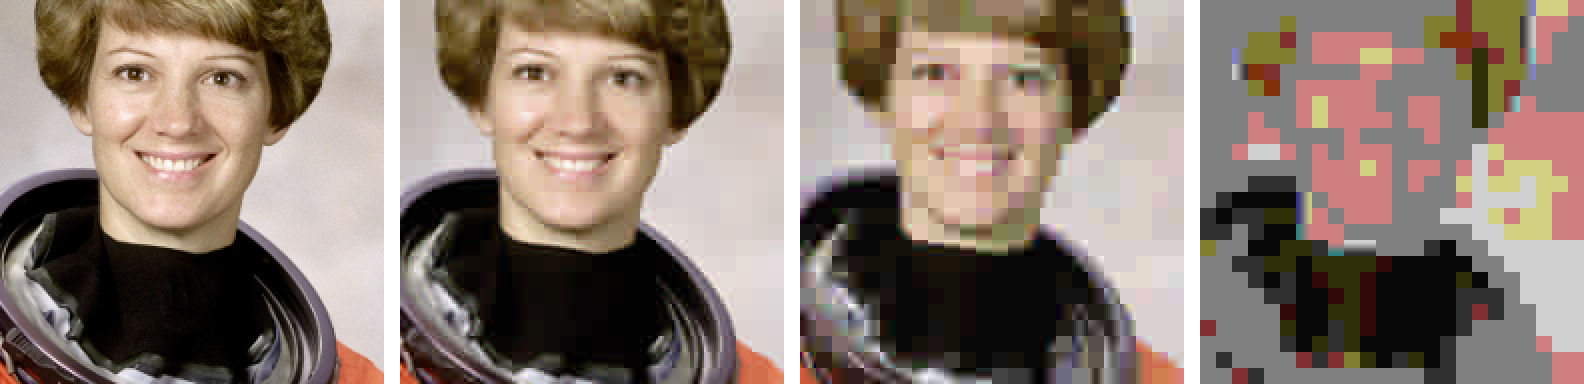
\includegraphics[width=0.94\textwidth]{figures/alpha.png}\\[0.1em]
  {\scriptsize
    \makebox[0.2374\textwidth]{originale}%
    \makebox[0.2374\textwidth]{$\alpha = 1$}%
    \makebox[0.2374\textwidth]{$\alpha = 5$}%
    \makebox[0.2278\textwidth]{$\alpha = 20$}}

  \vspace{0.6em}
  \small
  \begin{tabular}{@{}lrrrr@{}}
    \toprule
    & Conservation & Erreur $L^2$ & Taille CSR & Gain dense/CSR \\
    \midrule
    $\alpha = 1$ & 5,79\,\% & 5,43\,\% & 273\,Ko & 22,5 \\
    $\alpha = 5$ & 2,15\,\% & 11,29\,\% & 105\,Ko & 58,5 \\
    $\alpha = 20$ & 0,64\,\% & 32,95\,\% & 35\,Ko & 174,0 \\
    \bottomrule
  \end{tabular}
\end{frame}

\begin{frame}{Résultats : matrices de quantification}
  \centering
  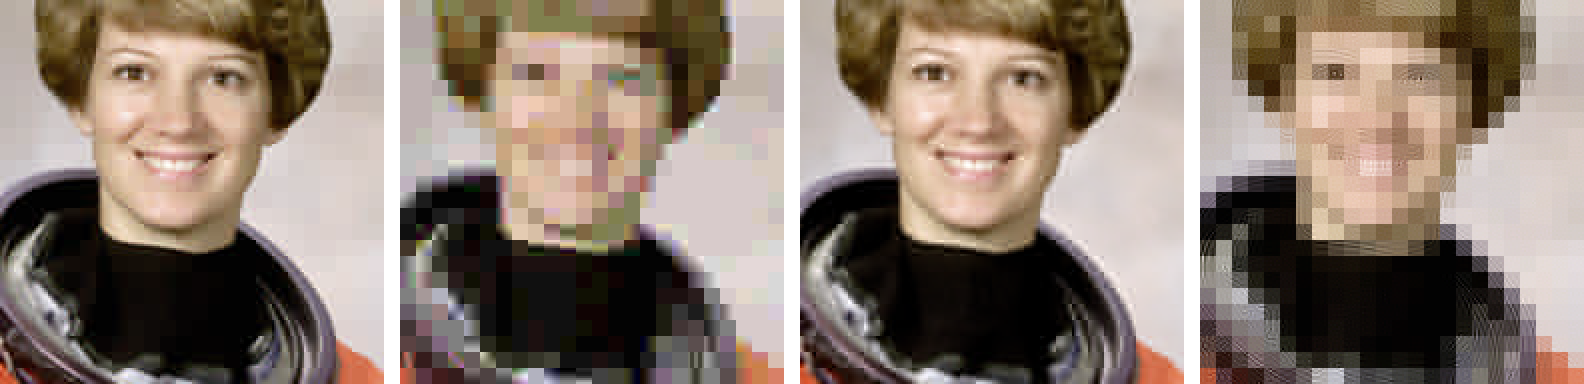
\includegraphics[width=0.9\textwidth]{figures/tables.png}\\[0.1em]
  {\scriptsize
    \makebox[0.2273\textwidth]{$Q$ standard}%
    \makebox[0.2273\textwidth]{$Q$ uniforme (100)}%
    \makebox[0.2273\textwidth]{basses fréquences}%
    \makebox[0.2181\textwidth]{hautes fréquences}}

  \vspace{0.5em}
  \small
  \begin{tabular}{@{}lrrr@{}}
    \toprule
    & Conservation & Erreur $L^2$ & Taille CSR \\
    \midrule
    $Q$ standard (psychovisuelle) & 5,79\,\% & 5,43\,\% & 273\,Ko \\
    $Q$ uniforme & 1,65\,\% & 13,85\,\% & 82\,Ko \\
    diviseurs faibles en basses fréquences & 8,76\,\% & 6,52\,\% & 409\,Ko \\
    diviseurs faibles en hautes fréquences & 25,45\,\% & 17,49\,\% & 1\,179\,Ko \\
    \bottomrule
  \end{tabular}
\end{frame}

\begin{frame}{Résultats : bruit poivre et sel}
  \centering
  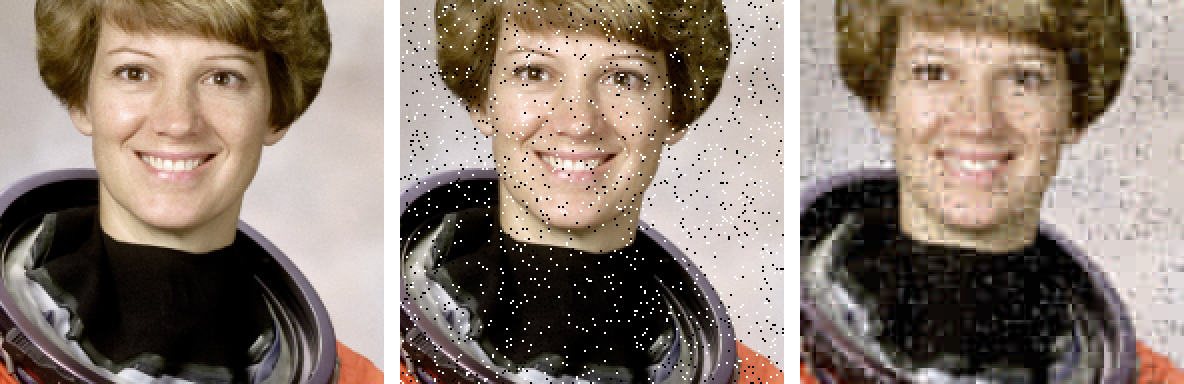
\includegraphics[width=0.8\textwidth]{figures/bruit.png}\\[0.1em]
  {\scriptsize
    \makebox[0.2703\textwidth]{image pure}%
    \makebox[0.2703\textwidth]{bruitée à 5\,\%}%
    \makebox[0.2594\textwidth]{reconstruite, masque triangulaire $F = 4$}}

  \vspace{0.8em}
  \begin{columns}[T]
    \begin{column}{0.44\textwidth}
      \small
      Erreur $L^2$ par rapport à l'image pure :
      \begin{itemize}
        \item image bruitée : 24,0\,\%
        \item reconstruite, triangle $F = 4$ : 11,3\,\%
        \item reconstruite, réglages Python : 12,8\,\%
      \end{itemize}
    \end{column}
    \begin{column}{0.44\textwidth}
      \small
      Le bruit est fait de variations très rapides, donc de hautes fréquences :
      la troncature agit comme un filtre passe-bas, au prix d'un flou des contours.
    \end{column}
  \end{columns}
\end{frame}

\begin{frame}{Validation et performances}
  \begin{columns}[T]
    \begin{column}{0.31\textwidth}
      \centering
      {\Huge\bfseries\color{accent} 17}\\[0.2em]
      \small fonctions de test\\[0.6em]
      \begin{itemize}
        \scriptsize
        \item tests pytest de la version Python
        \item invariants de chaque classe
        \item aller-retour par fichier \code{.csr}
        \item ligne de commande
      \end{itemize}
    \end{column}
    \begin{column}{0.33\textwidth}
      \centering
      {\Huge\bfseries\color{accent} 25}\\[0.2em]
      \small coefficients différents sur 786\,432\\[0.6em]
      \scriptsize
      Même nombre de non nuls (45\,566). En Python, $D/Q$ vaut
      $23{,}999\,999\,999\,999\,996$ au lieu de 24 (image passée par $/255$ puis
      $\times255$) : la troncature donne 23.
    \end{column}
    \begin{column}{0.31\textwidth}
      \centering
      {\Huge\bfseries\color{accent} $\times$11}\\[0.2em]
      \small plus rapide que Python\\[0.6em]
      \scriptsize
      Compression et décompression de $512\times512$ : 50\,ms en C++ contre 543\,ms en
      Python (même machine, meilleur de 3 essais).
    \end{column}
  \end{columns}
\end{frame}

\begin{frame}{Bilan et perspectives}
  \begin{columns}[T]
    \begin{column}{0.48\textwidth}
      \textbf{Bilan}
      \begin{itemize}
        \item toutes les fonctionnalités Python reproduites en C++20
        \item mêmes coefficients, onze fois plus vite
        \item invariants : dimensions, type \code{int16}, fichier CSR cohérent
        \item aucune gestion mémoire manuelle hors \code{StbPixels}
      \end{itemize}
    \end{column}
    \begin{column}{0.48\textwidth}
      \textbf{Perspectives}
      \begin{itemize}
        \item parcours zigzag et codage entropique (RLE, Huffman) : vrai fichier JPEG
        \item espace YCbCr et sous-échantillonnage de la chrominance
        \item plusieurs masques polymorphes avec \code{std::unique\_ptr}
      \end{itemize}
    \end{column}
  \end{columns}
  \vspace{1.2em}
  \centering
  \small \url{https://github.com/BnRomain/jpeg-compression}
\end{frame}

\end{document}
